\documentclass{sigchi}

% Use this command to override the default ACM copyright statement
% (e.g. for preprints).  Consult the conference website for the
% camera-ready copyright statement.


%% EXAMPLE BEGIN -- HOW TO OVERRIDE THE DEFAULT COPYRIGHT STRIP -- (July 22, 2013 - Paul Baumann)
% \toappear{Permission to make digital or hard copies of all or part of this work for personal or classroom use is      granted without fee provided that copies are not made or distributed for profit or commercial advantage and that copies bear this notice and the full citation on the first page. Copyrights for components of this work owned by others than ACM must be honored. Abstracting with credit is permitted. To copy otherwise, or republish, to post on servers or to redistribute to lists, requires prior specific permission and/or a fee. Request permissions from permissions@acm.org. \\
% {\emph{CHI'14}}, April 26--May 1, 2014, Toronto, Canada. \\
% Copyright \copyright~2014 ACM ISBN/14/04...\$15.00. \\
% DOI string from ACM form confirmation}
%% EXAMPLE END -- HOW TO OVERRIDE THE DEFAULT COPYRIGHT STRIP -- (July 22, 2013 - Paul Baumann)


% Arabic page numbers for submission.  Remove this line to eliminate
% page numbers for the camera ready copy 

%\pagenumbering{arabic}

% Load basic packages
\usepackage{balance}  % to better equalize the last page
\usepackage{graphics} % for EPS, load graphicx instead 
%\usepackage[T1]{fontenc}
\usepackage{txfonts}
\usepackage{times}    % comment if you want LaTeX's default font
\usepackage[pdftex]{hyperref}
% \usepackage{url}      % llt: nicely formatted URLs
\usepackage{color}
\usepackage{textcomp}
\usepackage{booktabs}
\usepackage{ccicons}
\usepackage{todonotes}
\usepackage{subfigure}
\usepackage{multirow}

% llt: Define a global style for URLs, rather that the default one
\makeatletter
\def\url@leostyle{%
  \@ifundefined{selectfont}{\def\UrlFont{\sf}}{\def\UrlFont{\small\bf\ttfamily}}}
\makeatother
\urlstyle{leo}

% To make various LaTeX processors do the right thing with page size.
\def\pprw{8.5in}
\def\pprh{11in}
\special{papersize=\pprw,\pprh}
\setlength{\paperwidth}{\pprw}
\setlength{\paperheight}{\pprh}
\setlength{\pdfpagewidth}{\pprw}
\setlength{\pdfpageheight}{\pprh}

% Make sure hyperref comes last of your loaded packages, to give it a
% fighting chance of not being over-written, since its job is to
% redefine many LaTeX commands.
\definecolor{linkColor}{RGB}{6,125,233}
\hypersetup{%
  pdftitle={SIGCHI Conference Proceedings Format},
  pdfauthor={LaTeX},
  pdfkeywords={SIGCHI, proceedings, archival format},
  bookmarksnumbered,
  pdfstartview={FitH},
  colorlinks,
  citecolor=black,
  filecolor=black,
  linkcolor=black,
  urlcolor=linkColor,
  breaklinks=true,
}

% create a shortcut to typeset table headings
% \newcommand\tabhead[1]{\small\textbf{#1}}

% End of preamble. Here it comes the document.
\begin{document}
\author{
  Yvonne Chen\\
  \texttt{evechen@uw.edu}
  \and
  Eleanor O'Rourke\\
  \texttt{eorourke@cs.washington.edu}
}
\title{Visualizing Student Problem-Solving Data}


\maketitle

\begin{abstract}
Abstract goes here
\end{abstract}


%\keywords{Technology in the classroom; tablets for education; adaptive learning environments.}

%\category{H.5.0.}{Information Interfaces and Presentation}{General}

\section{Introduction}
An explanation of the problem and the motivation for solving it.

\section{Related Work}
A large body of research has explored methods of integrating technology into in-person classrooms and using technology to deliver education online. We review this research focusing on technology-delivered curriculums, systems that expose student data for teachers, and adaptive learning environments.

\subsection{Exposing Student Data for Teachers}
Education research shows that teacher behavior has a strong impact on student achievement \cite{Hill2005, Wentzel2002, Reeve2004, Wright1997}, and that teachers can benefit from the availability of real-time student data \cite{Balaam2010, Koile2006, Lazar2007}. For example, Koile found that when an instructor was given access to student problem solutions through tablet-based technology in real-time, the instructor devoted 75\% of class time responding to student misunderstandings \cite{Koile2006}. With access to real-time data, research suggests that instructors can intervene during a lesson when students are confused \cite{Hickey2014}, alter the pace or content of instruction based on student engagement \cite{Balaam2010}, immediately identify and assist students who are struggling \cite{Lazar2007}, and choose topics of focus based on aggregates of student responses \cite{Koile2006}. 

A number of technologies have been developed for exposing student data for teachers. One technology that is often used in lecture-based classes is the ``student response system'' or ``clicker,'' which is used to poll students on multiple-choice questions during class \cite{Dangel08, Lazar2007}. A similar application designed for small classes is Plickers \cite{Plickers}. With the Plickers smartphone app, the teacher can scan the classroom while students hold up QR codes identifying a multiple-choice answer \cite{Plickers}. Researchers have also explored methods of providing instructors with access to student data outside of instruction time to monitor longer term academic progress \cite{Zhang2015, Arnold2012}. Kim et.\ al.\ developed a system for compiling student responses to MOOC exercise problems, which teachers reported were useful for capturing student thought processes, identifying misconceptions, and engaging students with content \cite{Kim2015}.

In this work, we explore methods of exposing rich problem-solving data to elementary school teachers in real-time. Through a longitudinal study, we explore how teacher behavior is impacted by exposing information about student misconnects and progress through curriculum material.

Whether viewed in real time or after the fact, teachers benefit from the availability of student data. Accessed in real time, student data affords immediate intervention. In a study by Koile, students used Tablet PCs to complete exercise problems during class time. The instructor could access their answers right away on her own device. Based on the students? answers, the instructor devoted 75\% of course time responding to misunderstandings of course material, and would delay or hasten presentation of new material as appropriate \cite{Koile2006}. With real time student data, instructors can intervene during a lesson when students are confused \cite{Hickey2014}, alter the pace or content of instruction based on student engagement \cite{Balaam2010}, immediately identify and assist students who are struggling \cite{Lazar2007}, and choose topics of focus based on aggregates of student responses \cite{Koile2006}.

When timely intervention is less critical, instructors can view data outside of instruction time to
monitor longer term academic progress \cite{Zhang2015, Arnold2012}. Kim et al developed an online system for teachers to author video lectures containing integrated multimedia exercises. The system compiled student responses as they completed exercises, and teachers reported that they were useful for ?capturing students? thought processes, identifying misconceptions, and engaging students with content? \cite{Kim2015}. Even basic classroom response systems, which poll students to choose one out of a set of pre-defined responses, give teachers a quick aggregate overview of student understanding \cite{Lazar2007}.

While research shows that student data can help teachers understand misconceptions and how they spend class time, very little is known about how to visualize student data to most effectively communicate with teachers. We have not encountered any papers that study the design of visualizations of student data. Enlearn has implemented two different methods of visualizing student data in real-time for teachers, however, both of their designs have had usability and readability problems when tested in classrooms. This shows how challenging it is to create effective visualizations for communicating student data in real-time. Enlearn?s first design, shown in Figure 1a, displays a table view of student problem solving pace and correctness. While this visualization provides information about the progress of individual students, it communicates nothing about the specific concepts that students are struggling with. Enlearn?s second design, shown in Figure 1b, displays a graph view of student problem solving that is organized by concept. While this displays information about the concepts that students are struggling with, there is no way for teachers to see which individuals are struggling. Most importantly, neither visualization provides teachers with actionable suggestions about how to assist students who are struggling. Prior work shows the utility of communicating student data for instructors, and Enlearn?s experiences with their current visualizations shows the challenge of designing effective means of communicating data, especially in real time for busy teachers. This motivates our desire to improve and strengthen the data visualization for the Enlearn software.

\section{Enlearn}
For this project, we partnered with Enlearn, a non-profit company founded to develop tablet-based adaptive problem-solving software for K-12 classrooms. In our visualizations, we display real data from Enlearn students.

Enlearn evaluated two visualizations with teachers this spring. One displays student data in a table view, but provides no concept-level information. The other displays a concept graph, but provides no data at the level of individual students.

Enlearn found that neither visualization was effective in the classroom, in large part because the information provided did not match teacher needs. Another challenge is that teachers are extremely busy during class time and need visualizations that are both easily glanceable and that provide actionable information.




\section{Methods}
To address the challenge of designing effective techniques for visualizing student problem-solving data for teachers, we first characterize the problem, then discuss our data abstractions, present our visual encodings for conveying the data, and describe our implementation.


\subsection{Problem Characterization}
The initial goal of this research was to understand the format of the problem-solving data collected by the Enlearn software and accurately characterize the tasks that teachers want to accomplish using this data. The challenges that Enlearn faced with their initial visualization designs shows the importance of understanding user needs; Enlearn's visualizations failed in large part because they did not effectively support teacher tasks. While we did not directly meet with teachers, we worked closely with Enlearn staff to understand the feedback they received in response to their initial visualizations. Here we first describe the structure of the problem-solving data collected by Enlearn, and then describe teacher tasks. We provide a set of design guidelines for our visualizations based on this problem characterization.

\subsubsection{Enlearn Data Structure}
In Enlearn classrooms, each student solves problems on a personal tablet. Enlearn logs the following problem-solving information to a database: the id of the student, the id of the problem, the id of the associated problem set, and whether or not the student answered the problem correctly. The Enlearn adaptive curriculum is designed as an extension of the JUMP Math curriculum \cite{JUMPMath}. In JUMP Math, students solve a linear progression of Exercise and Workbook problems. In Enlearn's adaptive version of the curriculum, students practice each type of Exercise or Workbook problem until they have mastered the concept covered by that problem. As a result, students may work on multiple practice problems of the type ``Exercise Problem 3'' before moving on to the next problem type. Enlearn refers to each problem type as a \emph{problem set}, but we use the term \emph{concept} in this paper since it better matches how teachers refer to the groups of problems.

\subsubsection{Teacher Tasks}
Through our discussions with Enlearn staff, we learned that there are two primary tasks that teachers want to accomplish using student problem-solving data during class. First, teachers want to determine which students need individual assistance and what specific concepts they are struggling with at any given moment. Ideally, teachers would also be able to see if multiple students are struggling with the same concept at the same time so that they can pull the students aside to work with them as a group. Second, teachers want to determine how each student is performing overall during the current lesson. If many students are struggling with the content, the teacher may chose to re-teach parts of the lesson.

While Enlearn's initial visualizations tried to target these tasks, they did not provide adequate information for teachers to be able to quickly determine which students were struggling the most and what concepts they were currently working on. The overwhelming feedback that Enlearn was given by teachers after their trial was that the real-time visualizations need to provide information that is glanceable and immediately actionable. During class, teachers are busy adapting lessons, responding to students, and managing organizational challenges. They do not have time to explore a complex visualization of student data. Instead, they need a simple view that provides them with the exact information they need to accomplish in-class tasks such as assisting students and adapting their teaching strategy.

\subsubsection{Design Guidelines}
From our characterization of the structure of Enlearn's problem-solving data and the tasks that teachers need to accomplish using that data, we developed the following design guidelines for our visualizations:

\begin{itemize} \itemsep5pt \parskip0pt \parsep0pt
  \item Visualizations must provide actionable information that clearly displays student performance on practice problems.
  \item Visualizations must show data for individual students so that teachers can easily intervene when needed.
  \item Visualizations must display concept-level data so that teachers can assess student understanding of each concept.
\end{itemize}

We use these guidelines throughout the remainder of our work focus our data abstraction and visual encoding designs.


\subsection{Data Abstractions}





\subsection{Visual Encodings}

\subsubsection{Simulating Real-Time Data}
Our visualizations are designed to display real-time student data, however we do not have a constant stream of data to display. To simulate real-time problem solving, we use data collected from students last fall. We display a timeline that can be played and brushed to allow both us and the Enlearn staff to quickly see what the visualizations would look like in a variety of real-time scenarios. We display lines on the timeline showing where problem-solving actions occur, so the viewer can easily become acclimated to the data set. While we designed this feature for our benefit as designers, it may be valuable for teachers to play back their lessons.


\subsubsection{Concept View}
The concept visualization is designed to help teachers determine which students need help in the present moment. Students are grouped by the concept that they are currently working on so that it is easy for the teacher to know what concept to target. The background color of each student bar indicates how well the student is performing on that concept. This view gives teachers a glanceable display that can help them rapidly determine which student to assist.

\subsubsection{Aggregated View}
The aggregate visualization is designed to give teachers a high-level overview of how each student has performed over the course of the lesson. This view displays all problem-solving information for each student across multiple concepts. The background is colored to show the student�s aggregate performance.  If the teacher wants to see concept-level information for a given student, she can click on that student to see the individual visualization shown to the right above.



\subsubsection{Visualization Options}

\subsection{Implementation}

\section{Results}
The visualizations your system produces and data to help evaluate your approach. For example you may include running times, or the time users typically spend generating a visualization using your system.

%\begin{figure*}[t]
%\centering
%\subfigure[]{\label{fig:TeacherLesson}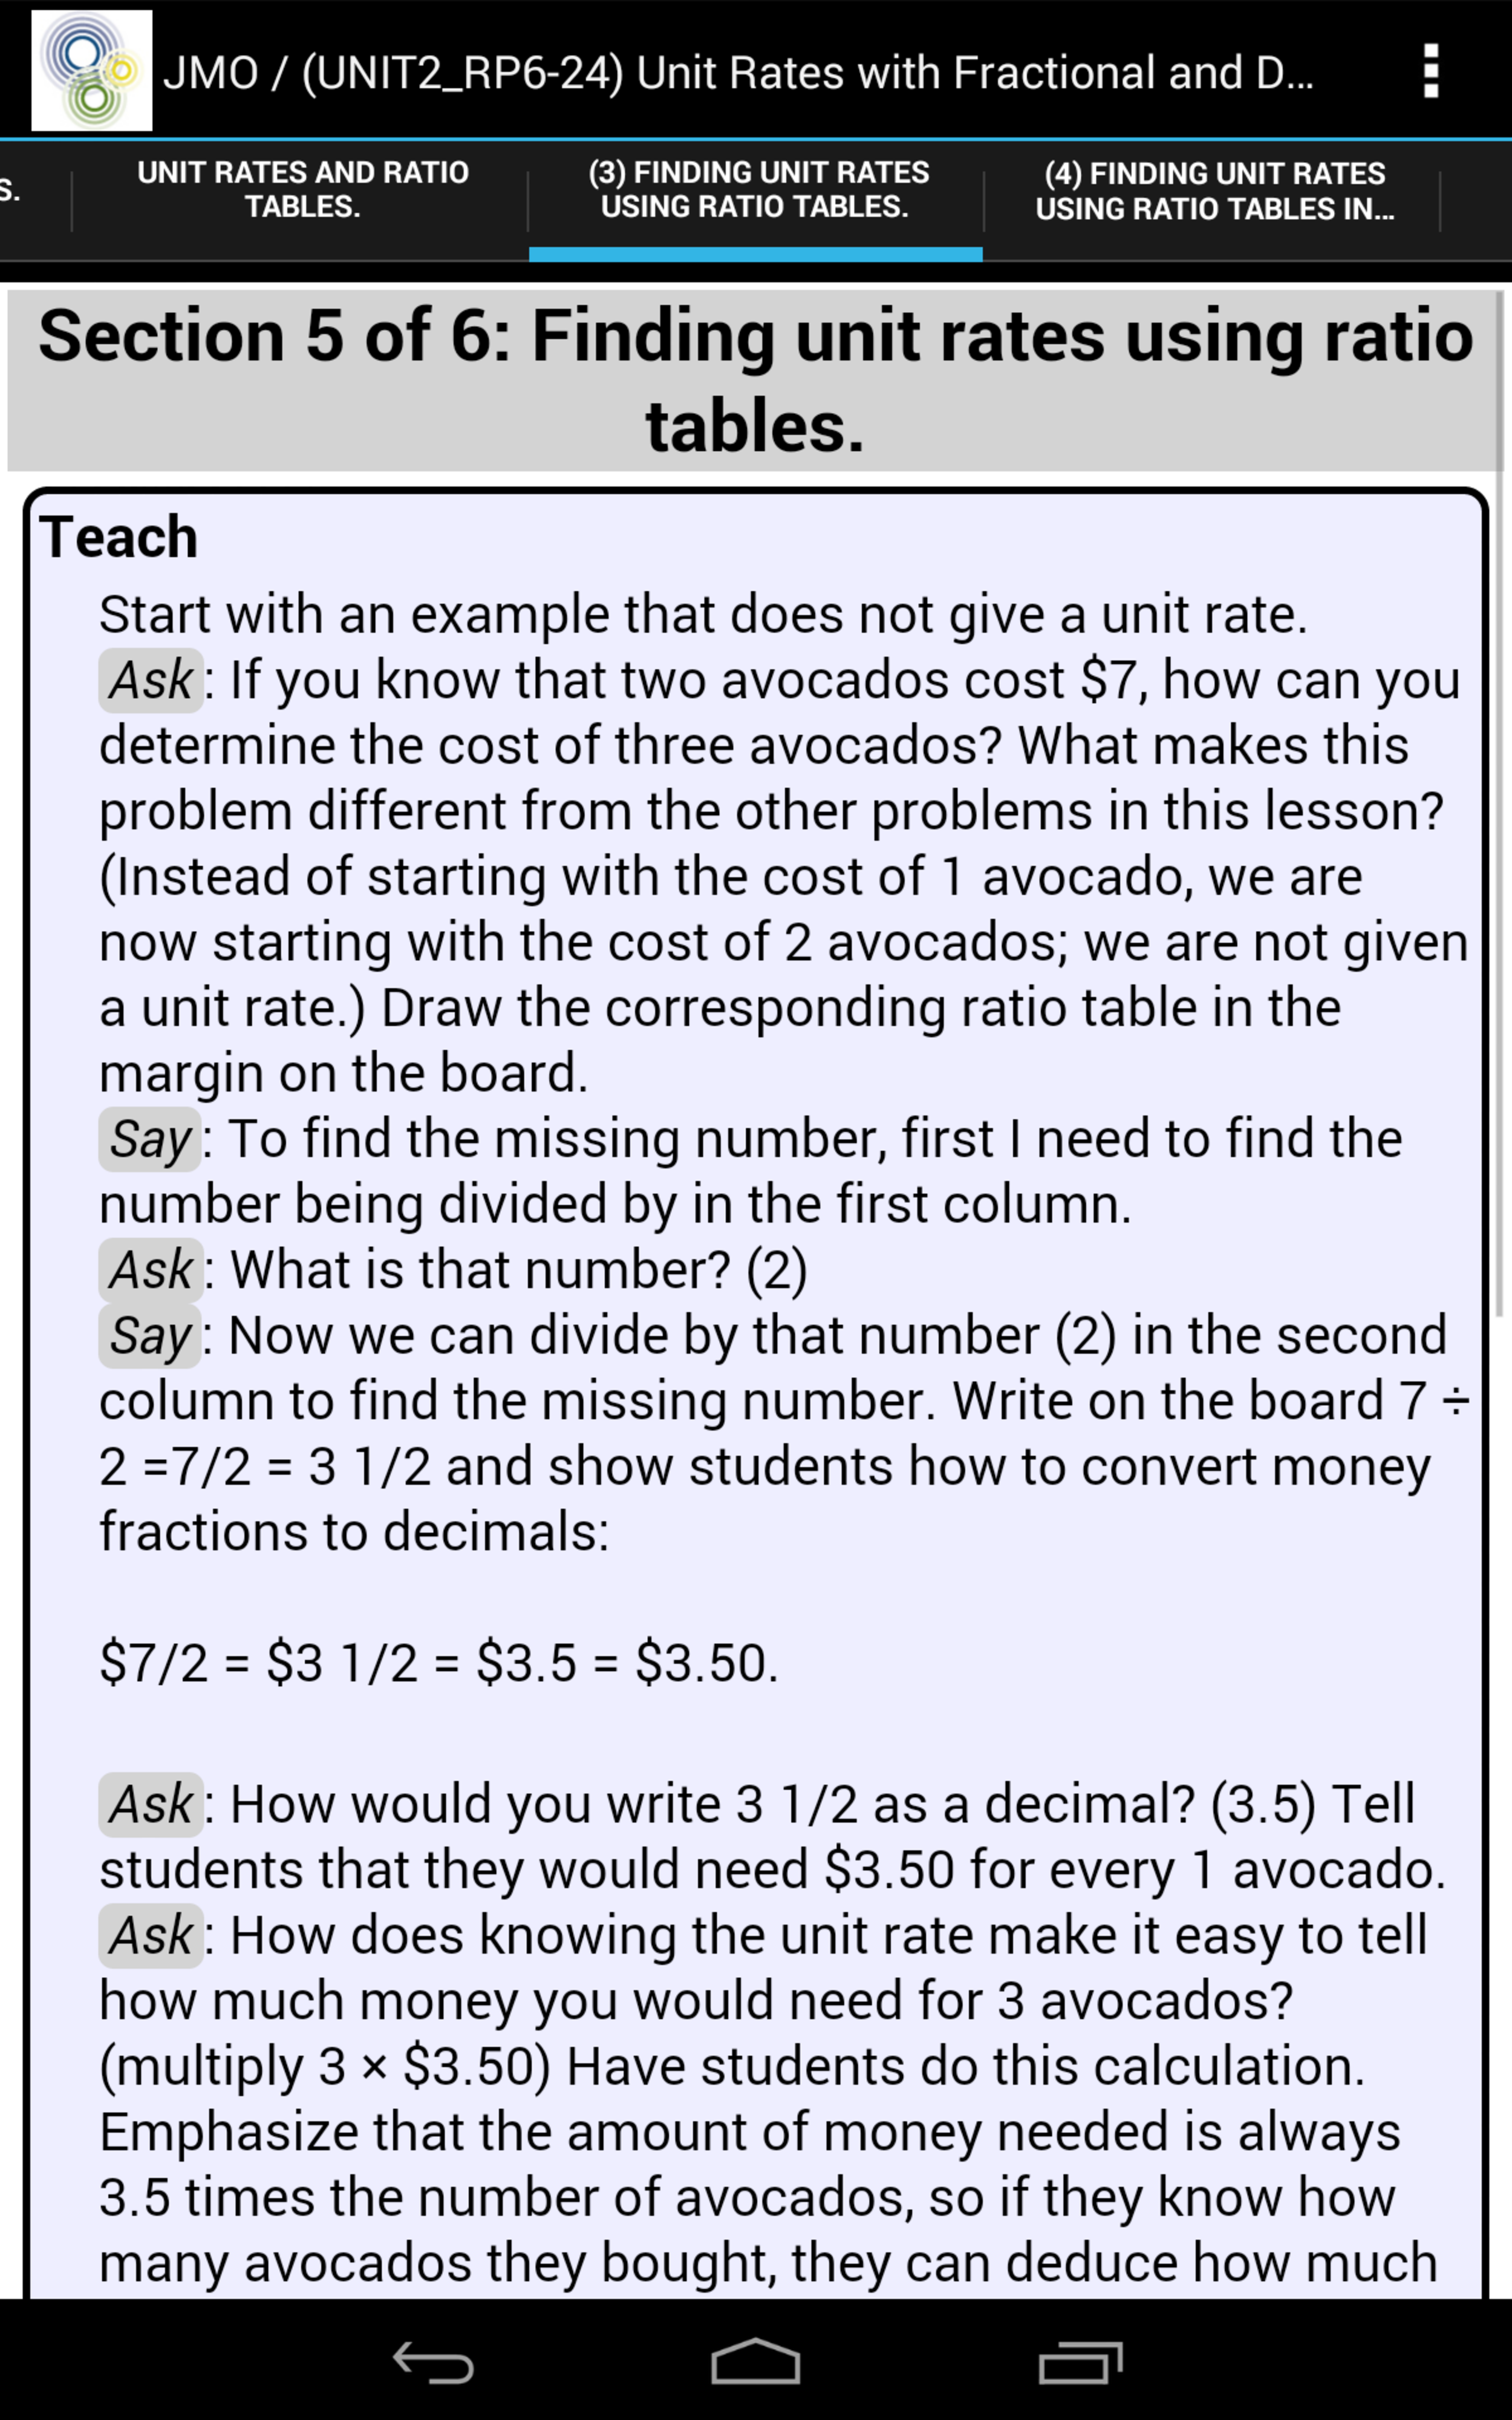
\includegraphics[width=40mm]{images/TeacherLesson.pdf}} \hspace{1em}%
%\subfigure[]{\label{fig:TeacherStartProbems}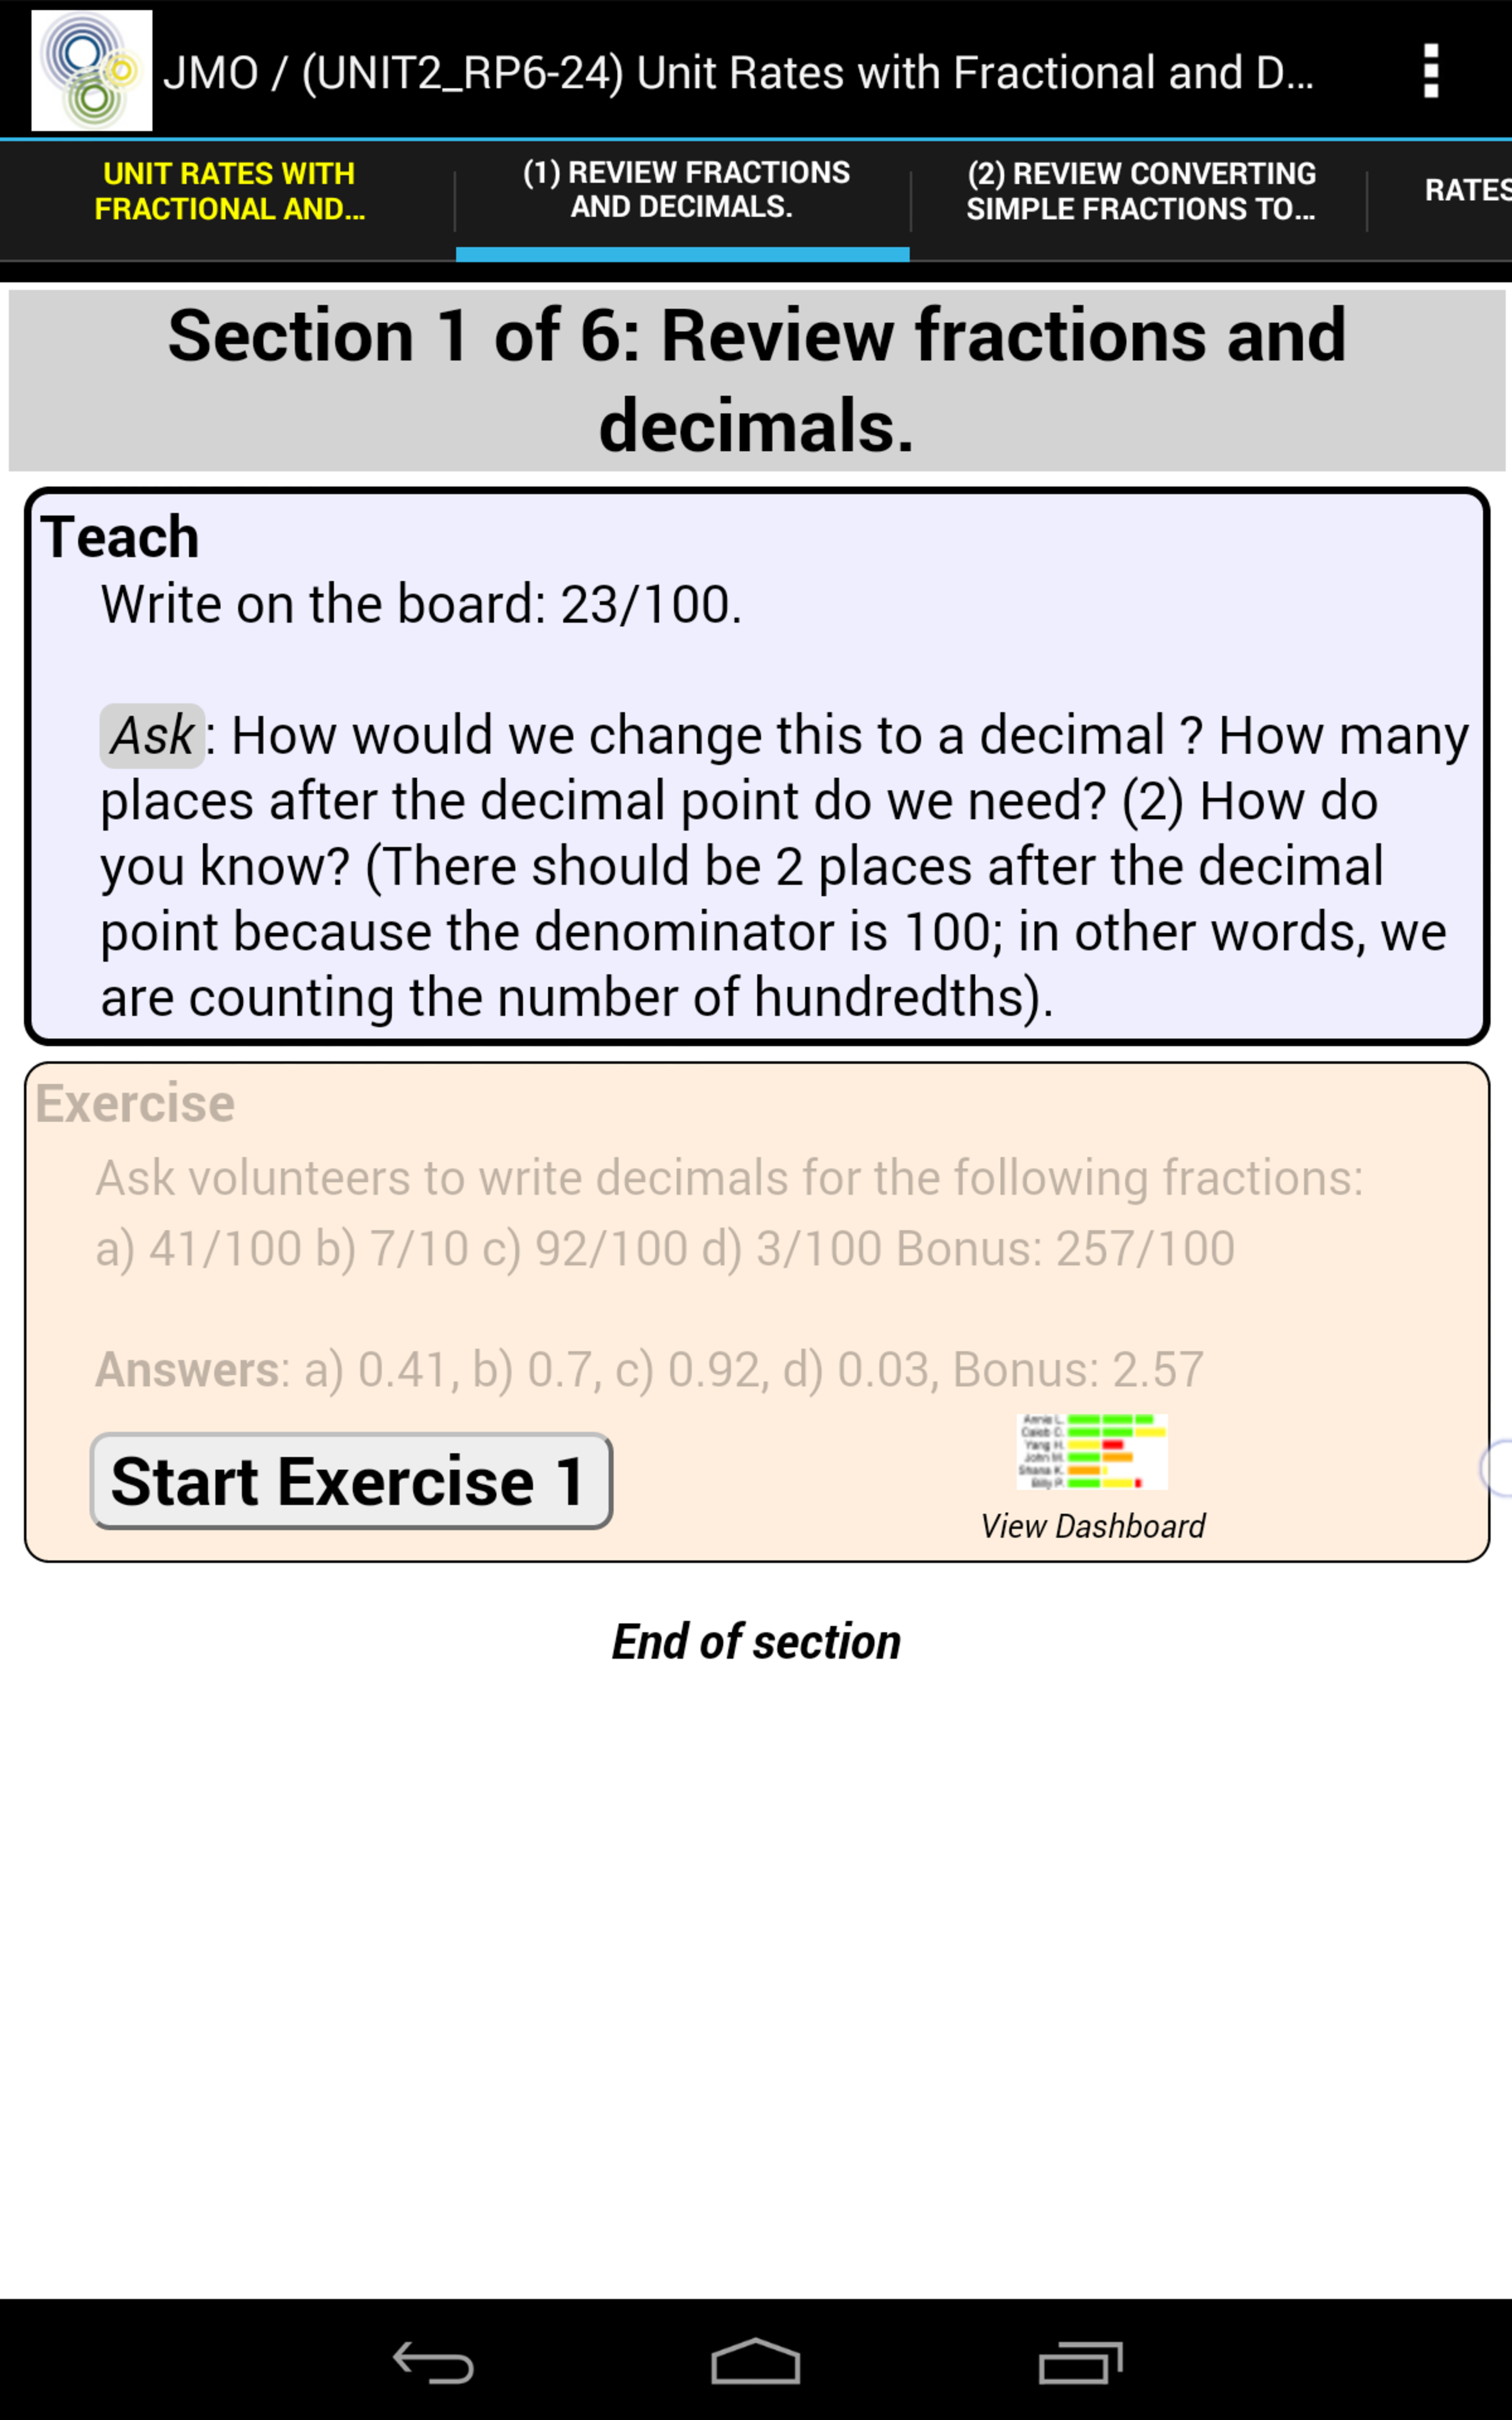
\includegraphics[width=40mm]{images/TeacherEX.pdf}} \hspace{1em}%
%\subfigure[]{\label{fig:TeacherDashboard}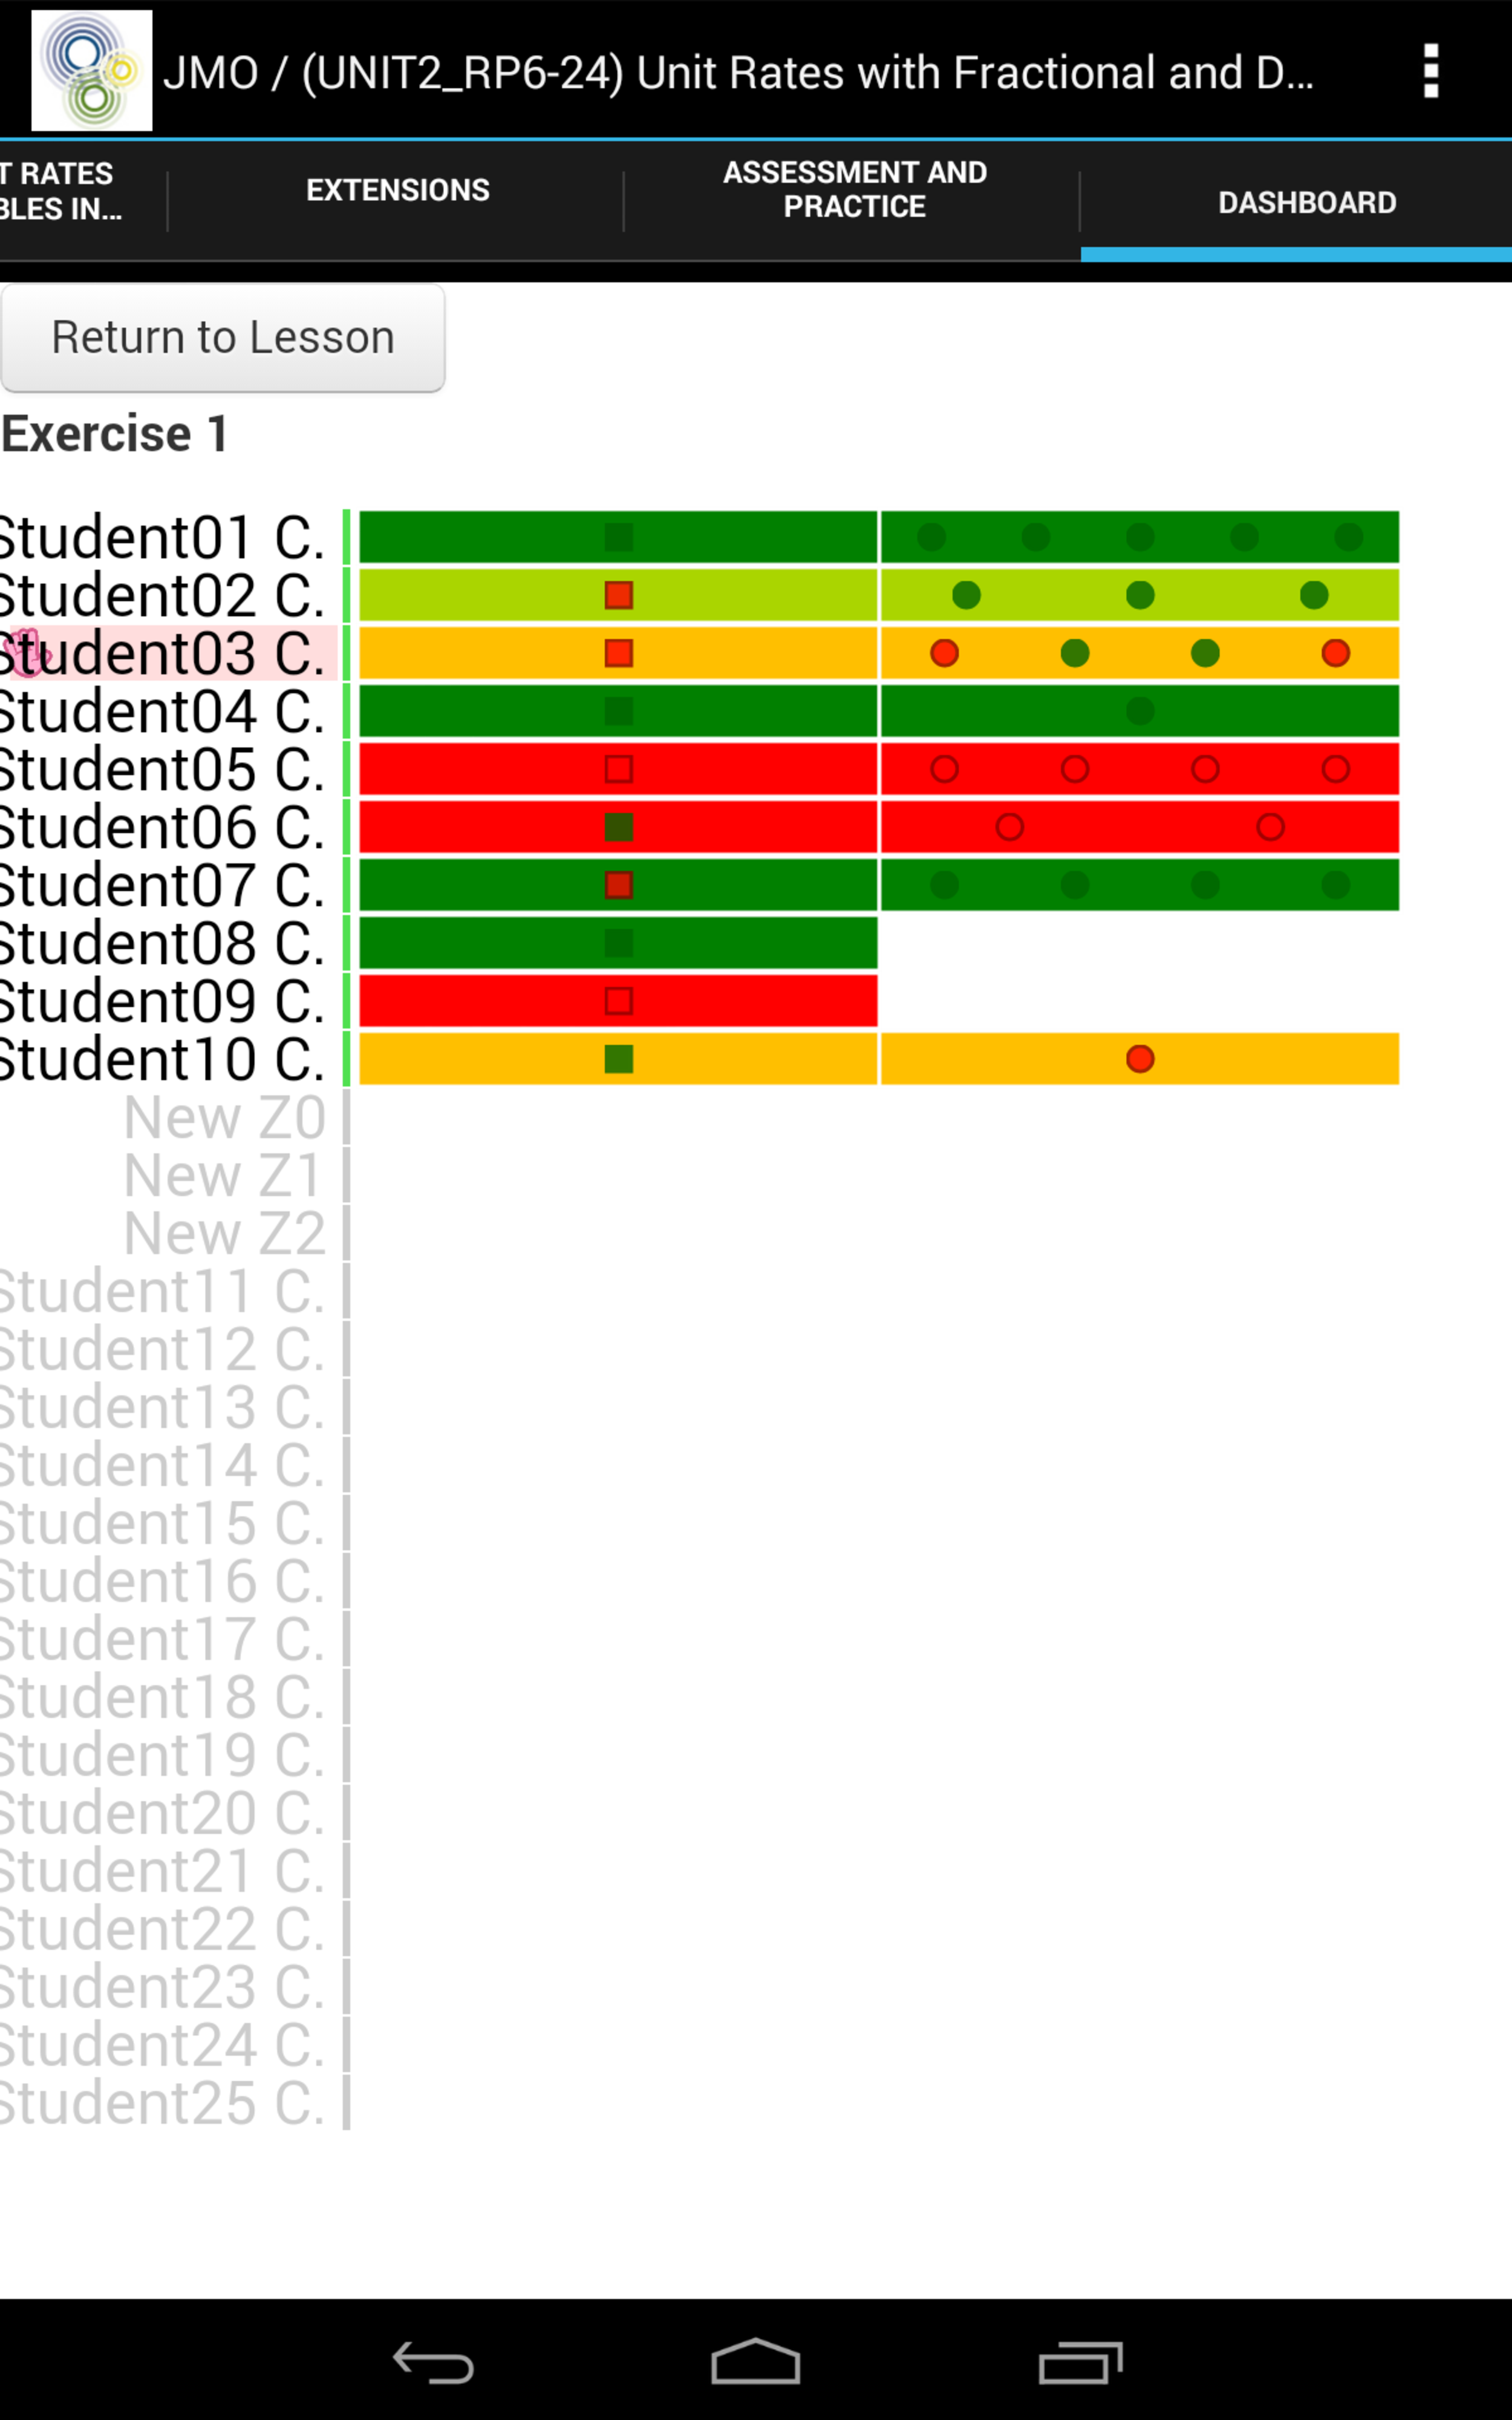
\includegraphics[width=40mm]{images/TeacherDashboard.pdf}} \hspace{1em}%
%\subfigure[]{\label{fig:StudentProblemSolving}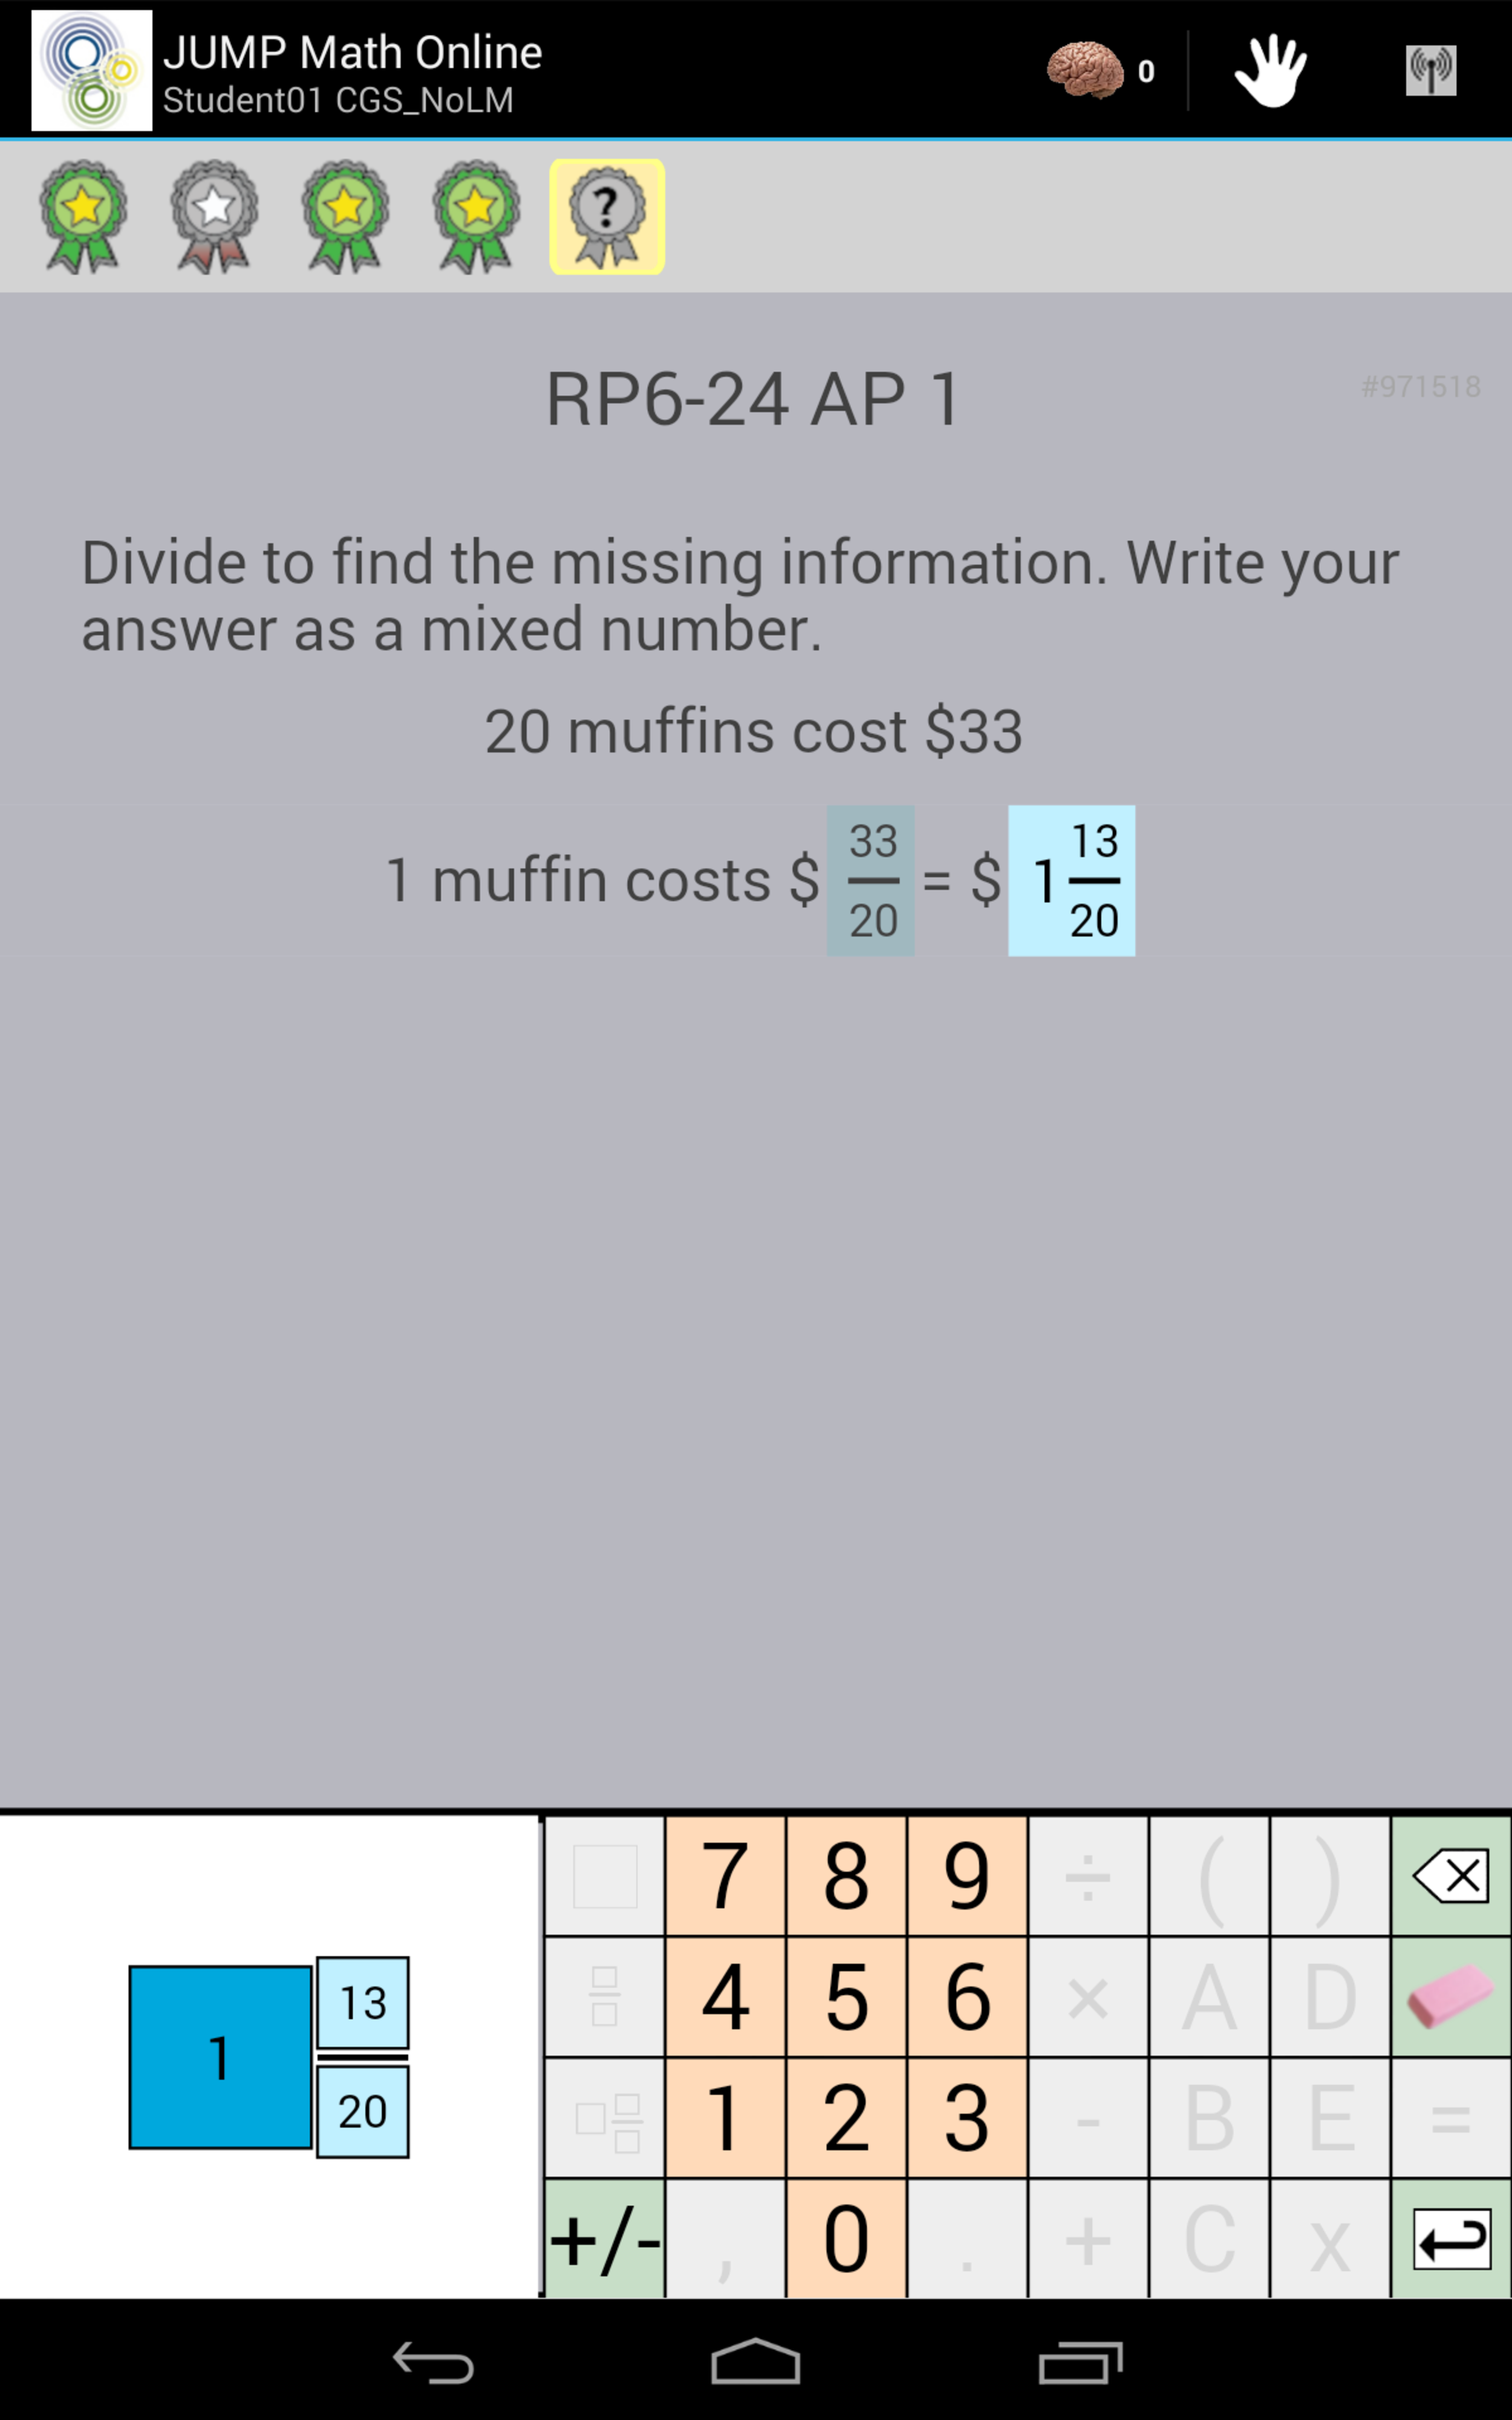
\includegraphics[width=40mm]{images/Student.pdf}}
%\caption{
%Screenshots of the Teacher and Student software. Figure (a) shows the teacher lesson view. Figure (b) shows a prompt for the teacher to ``Start Exercise 1'' on all student tablets. Figure (c) shows the teacher Dashboard that displays student problem-solving progress. Figure (d) shows the student problem-solving interface, with a calculator input interface at the bottom of the screen and badges at the top that indicate problem correctness. }
%\label{fig:Spreadsheet}
%\end{figure*}

\section{Discussion}
What has the audience learned from your work? What new insights or practices has your system enabled? A full blown user study is not expected, but informal observations of use that help evaluate your system are encouraged.

\section{Future Work}
A description of how your system could be extended or refined.

\section{Conclusion}



% Balancing columns in a ref list is a bit of a pain because you
% either use a hack like flushend or balance, or manually insert
% a column break.  http://www.tex.ac.uk/cgi-bin/texfaq2html?label=balance
% multicols doesn't work because we're already in two-column mode,
% and flushend isn't awesome, so I choose balance.  See this
% for more info: http://cs.brown.edu/system/software/latex/doc/balance.pdf
%
% Note that in a perfect world balance wants to be in the first
% column of the last page.
%
% If balance doesn't work for you, you can remove that and
% hard-code a column break into the bbl file right before you
% submit:
%
% http://stackoverflow.com/questions/2149854/how-to-manually-equalize-columns-
% in-an-ieee-paper-if-using-bibtex
%
% Or, just remove \balance and give up on balancing the last page.
%
%\balance{}


% REFERENCES FORMAT
% References must be the same font size as other body text.
\bibliographystyle{SIGCHI-Reference-Format}
\bibliography{references}

\end{document}

%%% Local Variables:
%%% mode: latex
%%% TeX-master: t
%%% End:
